% !TEX root =./main.tex

\section{Block 6: Quadrature Demodulation - Chen \& Stentiford}

The quadrature demodulator is used to detect the pulse envelopes. It is a type of 
amplitude modulation (AM) decoder which is able to function without knowing the exact 
phase of the signal's carrier wave. demodulation allows us to remove the carrier frequency
to recover the echo signal.

\subsection{Implementation}

Quadrature demodulation consists of three stages: mixing, filtering, and magnitude calculation.

\subsubsection{Mixing}

The mixing stage of a normal (synchronous) demodulator multiplies the received signal 
by the original carrier wave, matching the frequency and phase. Because we do not know 
the phase in this case, we instead split the incoming signal, multipling each copy by 
carrier waves 180° apart. Or, in mathematical terms:

\begin{align*}
    y[n] = x[n]*(\cos(2 \pi f n)+j \cos(2 \pi f n+\pi)) = x[n]*(\cos(2 \pi f n)+j \sin(2 \pi f n))
\end{align*}


To mitigate the relative slowness of trigonometric calculations, we pre-computed a pair of 
tables for cosine and sine which could be used in the actual block instead of calls to 
MATLAB's cosine and sine functions. The tables additionally already account for the sampling 
rate and carrier frequency in order to minimize multiplication operations inside the time-
sensitive block.

\subsubsection{Low-Pass Filtering}

Due to the mixing stage, frequency components are generated centering around both the original
carrier frequency and twice the carrier frequency (2fc). To isolate the desired carrier
frequency information, a low-pass filter (LPF) is used to suppress the high frequency components
generated around 2fc, leaving us with only the carrier frequency. The low-pass filtering ensures
that our demodulation output captures the original signal and not any duplicates of it.

Our low-pass filtering process utilizes the provided Blackman Rectangular filter. This LPF provides 
a steep drop-off which is ideal for isolating and extracting the DC components of the echo signal.

\begin{figure}[H]
    \centering
    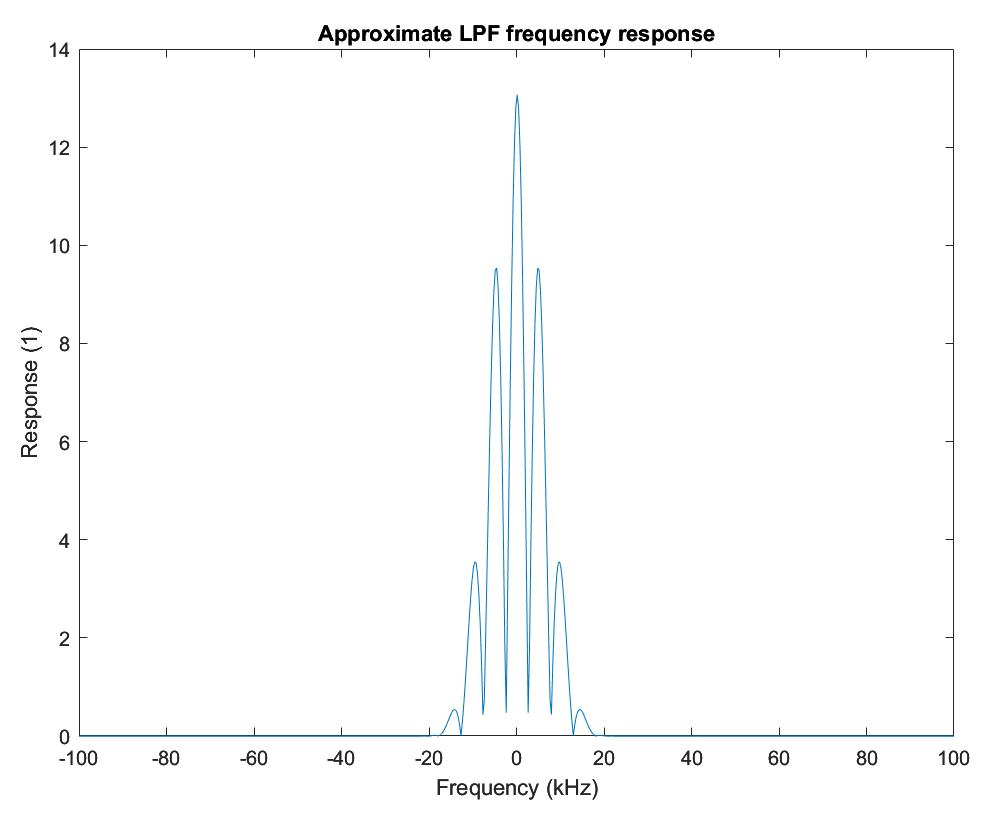
\includegraphics[width=0.5\linewidth]{figures/quad_lpf.png}
    \caption{Blackman LPF in the Frequency Domain}
    \label{fig:blackman_lpf}
\end{figure}

As shown in Figure 1, the Blackman LPF effectively attenuates all frequencies above the carrier
frequency of 10kHz. Beyond 20kHz, the filter eliminates all remaining frequencies, ensuring a 
clean signal within our desired range of DC components.

To make this stage more efficient, we preallocated arrays for the signals in-phase and quadrature
components. This approach eliminates the need to dynamically resize arrays during each iteration,
improving overall execution speed.


\subsubsection{Magnitude}

After filtering, the echo image is computed by taking the magnitude of the signal: 

\begin{align*}
    Y = \sqrt{I^2 + R^2}
\end{align*}

This allows us to merge the imaginary and real components back into a single envelope.

This is achieved as a single-line vector operation, and so is very performant.